\hypertarget{ClassFile_8cpp}{}\section{Referência ao ficheiro src/\+Class\+File.cpp}
\label{ClassFile_8cpp}\index{src/\+Class\+File.\+cpp@{src/\+Class\+File.\+cpp}}


Classe que irá realizar a leitura do bytecode e salvar as informações do class file.  


{\ttfamily \#include \char`\"{}Class\+File.\+h\char`\"{}}\newline
Diagrama de dependências de inclusão para Class\+File.\+cpp\+:\nopagebreak
\begin{figure}[H]
\begin{center}
\leavevmode
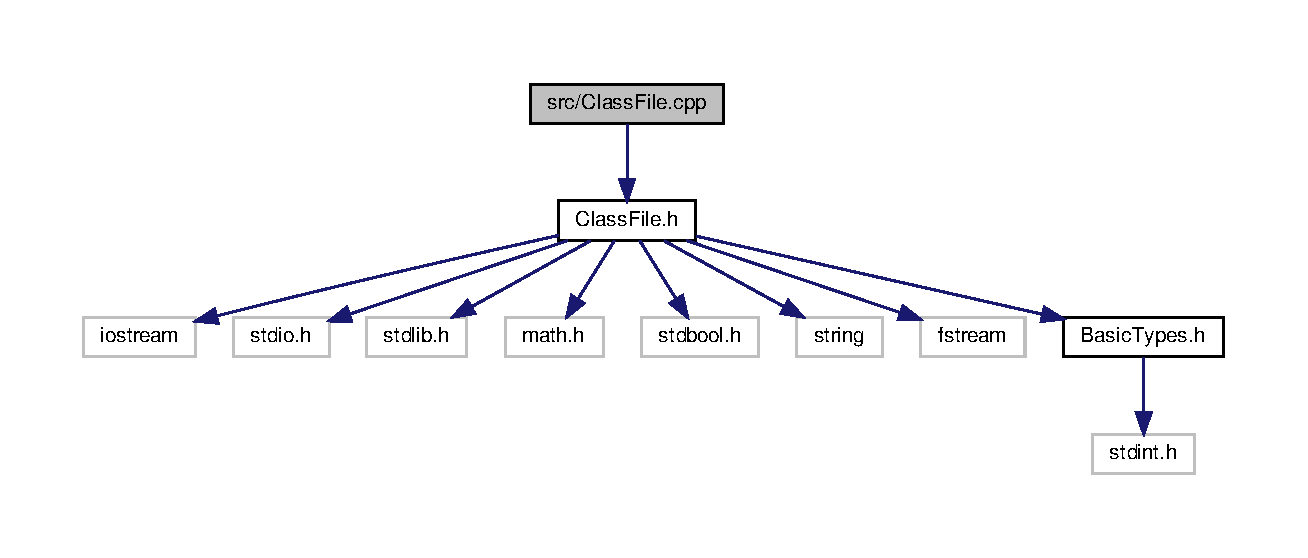
\includegraphics[width=350pt]{ClassFile_8cpp__incl}
\end{center}
\end{figure}


\subsection{Descrição detalhada}
Classe que irá realizar a leitura do bytecode e salvar as informações do class file. 

